\chapter{Introduction}
\label{ch:intro}
\chaptermark{Introduction}

%\setcounter{equation}{0}
% ==========================================================================================================

Recent advance on studies of on-going thought is driven by the popularisation of functional magnetic resonance imaging (fMRI), combined with established psychological researches. The increasing researches showed heterogeneous views on how and why mind wandering occurs, however the underlying mechanism is rather unexplored. The current thesis explores the patterns of on-going thought extending from well-studies category---mind wandering---to task-related thought. The aim is to gain an understanding of the component processes of on-going thought at task and rest. A flexible family resemblance view \cite{Seli2018} of on-going thought will joint the identified patterns of the shared similarities, as well as unique features that drives the heterogeneity.

In this chapter, I walk through the conflicting behavioural literature of mind wandering and discuss the theoretical accounts of on-going thought. Next I introduce the emerging neural evidence on hierarchical organisation that suggests how overlapping component processes might facilitate on-going thought. In closing, I introduce the overall methods used in the current research and how a multivariate approach helps to examine the family resemblance view.

\section{Heterogeneity of on-going thought}
\label{ch:intro:heterogeneity}
\sectionmark{Heterogeneity}

% lay out the component processing account and family resemblance view

With the advance of fMRI and other neuroimaging technique, the study of on-going thought has gained wider interest in psychology and neuroscience in the past decade. Mind wandering is particularly well-studied among all phenomena related to on-going thoughts. Researchers aim at understanding how the mind shifts between external environment and internal thoughts unrelated to the here-and-now. 
The executive failure account is concerned with why some mind wandering episodes occur to the detriment of the integrity on-going task. In contrast to the executive failure view, the representational account seeks an understanding of how the mental content is generated. The two approaches have led to a conflicts in the mind wandering literature. In a family resemblance view, members of the on-going thought family can have shared similarities along with unique features resulting the heterogeneity. The following section will introduce the evidence for construct overlap and shared processes of on-going thought at task and rest.

\subsection{Heterogeneity in definitions}
Among types of on-going thought, mind wandering attracted the most interest as it concerns the ability to focus on task at hand. Mind wandering has been studied in a variety of related psychological domains, such as cognition, emotion, and neuroscience. Various lines of research have addressed the basic phenomenal characteristics of mind wandering---
\begin{quote}
    \textit{a shift in the contents of thought away from an ongoing task and/or from events in the external environment to self-generated thoughts and feelings.}\\    
    \cite{SmallwoodSchooler2006,SmallwoodSchooler2015}.
\end{quote}
We are all familiar with moments when the train of thought shift away from the tasks at hand, and sometimes getting annoyed by the mind wandering episode. The intuition has lead to researches describing mind wandering as an `attentional lapse' \cite{McVayJOEP2009, McVay2012}, implying the occurrence of mind wandering is an unintended failure. When the study explicitly instruct the participant to perform a task, the time not focusing on the task are considered as `mind wandering'. Such research design dismissed the possibility of voluntary engagement of the mind wandering state. 

Recent investigations have found that mind wandering can occur with or without intention \cite<see review from>{SeliTiCS2016}. The participant can intentionally mind wander if they lack a motivation to engage in the experiment. When a simple yes/no question is asked about the mind wandering state, the response cannot access the nature of the occurrence. When participants are asked about the nature of mind wandering period in laboratory scenario, less than half of the mind wandering period is intentional \cite{SeliJoEP2015}due to the lack of motivation to complete the task \cite{SeliJoEP2015}, or the task is not mentally demanding to have all the attention resource allocated to the task \cite{SeliPsychScience2016}. The occurrence of intended and unintended mind wandering can also be down to individual differences. Intentional and unintentional mind wandering have been found to be deferentially associated with attention-deficit/hyperactivity disorder \cite<ADHD;>{SeliADHD2015} and obsessive-compulsive disorder \cite<OCD;>{SeliOCD2017}. The work on the intention of mind wandering demonstrates that there is indeed overlap in the various definitions, and that other components that contribute to the heterogeneity. 

\subsection{Heterogeneity in functional outcomes}

The family resemblance view suggests that complex thought can emerge from the combination of multiple overlapping processes. A myriad of mind wandering researches concern the functional outcomes. The current thesis proposes that the heterogeneous functional outcomes are evidence in support of a variety of component processes underlying the on-going thought. 

Mind wandering has been associated with poor executive control during working memory task \cite{McVayJOEP2009}. Individuals who mind-wandered more during fluid intelligent testing perform less well \cite{MrazekJoEP2012}. Mind wandering leads to bad reading comprehension due to failure in the construction of the mental models of ongoing events \cite{Smallwood2008}. Comprehension ability is related to working memory capacity and mediated by the ability to suppress mind wandering \cite{McVayReading2012, Unsworth2013}. Mind wandering has been linked to unhappiness \cite{Killingsworth2010} and a indicator of depression \cite{Smallwood2007}. The evidence above supported the highly disruptive nature of mind wandering and its potential costs to cognitive performance.

In addition to exploring the costs of mind wandering, researchers have discovered its potential benefits. Mind wandering may facilitate creative solution to an old problem \cite{Baird2012, Smeekens2016} and recovery from negative emotional states \cite{RubyPlos2013, PoerioFrontiers2016}. Mind wandering relays on mental time travel---the metal capacity of remembering the past and imagining the future \cite{Stawarczyk2015}.  Mind wandering can refine personal goals \cite{Medea2016} and is associated with the neural mechanism supporting mental time travel \cite{DArgembeau2006,DArgembeau2015}. 

Different functional associations arise from the same type of experience---mind wandering. To reconcile this contradictory evidence, researchers have suggested that mind wandering may encompasses multiple states with differential contents and underlying cognitive architectures \cite{SmallwoodFrontiers2013}. Complex thought can emerge from the combination of multiple overlapping processes. 

\subsection{Heterogeneity in experiential profiles}

Self-report is commonly used to understand the content of mind wandering thoughts and on-going experience. The content of mind wandering has a wide variety of topics and modality. The questions in the report address a number of dimensions of the on-going experience, ranging from the state of attention, temporal content, social content and modality. Principle component analysis (PCA) formalised the statistically shared association between the different aspects of the reports. 

Studies using PCA on such experience reports have revealed more detailed experiential profiles. Temporal information is one common theme \cite{RubyFP2013,RubyPlos2013}. The content of mind wandering is mainly future-focused \cite{Baird2011}, therefore mind wandering often involves planning for the future goals of the individual. On the contrary, when the mind wanders in an unhappy mood, the content is drawn to events from its past \cite{Smallwood2011}. The form of spontaneous thoughts is likely to be imagery or verbal \cite{Gorgolewski2014,Smallwood2016}. 

The positive/negative-valence of emotion of thought has tendency to accompany with different temporal directions. These unique associations discovered through PCA suggested the component processes at a experiential level. Investigation in experiential profiles is the first step to explore the commonality of various type of on-going thought. 

% ==========================================================================================================

\section{Theoretical accounts of mind wandering}
\sectionmark{Theoretical accounts}
\label{ch:intro:accounts}

The heterogeneity of mind wandering has been formalised into two theoretical accounts. The executive failure account aim to understand the conditions that trigger or associate with on-going thought. Researches on the mechanism behind the occurrence of on-going thought is the representational account. In other words, the executive failure account examines why changes in on-going thought happens, while the representational account interests in how human generates on-going thought while mind wandering. The two accounts can been seen as competing theories of mind wandering. However, in a family resemblance view, the two theoretical account supports the idea that the potential of a singular phenomenon is composed of multiple underlying component processes. 
\subsection{Executive failure account}
The executive failure account is concerned with a single aspect of mind wandering, namely understanding why some mind wandering episodes occur to the detriment of the integrity on-going task. Mind wandering occurs during attention-demanding tasks when control processes are insufficient to deal with the interference created by off-task thoughts \cite{Kane2012,McVay2010}. Mind wandering results from a failure of executive control over internally generated thoughts, rather than as consuming executive resources. The researches focus on the negative effect of mind wandering on the development of negative mood and task performance. Mind wandering thoughts are mostly unhappy in ecologically valid scenario \cite{Killingsworth2010}. Depressive thinking correlates with the frequency of mind wandering \cite{Smallwood2007}. 

In the executive failure view, mind wandering reflects momentary lapse in attention. The definition of attention lapse is a relatively slow response time to the task at hand, which is consistent with the mind wandering indicator used in working memory capacity research \cite{McVay2012}. Mind wandering has been considered the reason of poor executive control during working memory task \cite{McVayJOEP2009}. Executive error and slow reaction time correlates with individual differences in working memory capacity and mind wandering \cite{McVay2012}. The capacity to avoid mind wandering during demanding tasks is a potentially important source of success on measures of fluid intelligence \cite{MrazekJoEP2012}. 

% neural basis
Task-based fMRI study on attention lapse has contributed the functional neural processes to support the executive failure account. \citeA{Weissman2006} have uncover the neural mechanism behind the attention lapse during a global/local selective-attention task. Brief attention lapse is related t early activity in frontal control region including anterior cingulate cortex (ACC), right middle frontal gyrus (MFG), and right inferior frontal gyrus (IFG). Attention laspse also suggested the failure of maintaining perceptual representation. Reduced activity is found in primary visual area. Activation of default mode network \cite<DMN; >{Raichle2001} has been observed during a brief attention lapse. DMN is a set of brain regions composed of medial prefrontal cortex(MPFC), and posterior cingulate coretex (PCC) as the core and subsystems on medial and lateral regions of the temporal lobe. DMN is commonly referred as a task-negative network\cite{Fox2005}, associating with task-unrelated thought and mind wandering \cite{MasonScience2007,Christoff2009}. The lapses leads to demands on the frontal-parietal control relate regions for redirecting attention. Ventral frontal-parietal regions, including right temporal-parietal junction (TPJ) and right IFG, for recovery from lapses. 

\subsection{Representational account}

The representational account concerns the generation of content during mind wandering, suggesting that mind wandering is merely a mindless state. The ability to generate information without task-constrains is consistent with the productive functional outcomes of mind wandering, such as creativity \cite{Baird2012,Smeekens2016} and social-temporal problem solving \cite{RubyPlos2013,PoerioFrontiers2016,Medea2016}. 

Internal representation of semantics and episodic memory is associated with brain regions highly overlapped with DMN. The brain regions involved in semantic processing includes angular gyrus (AG), lateral and ventral temporal cortex, left dorsal MPFC, left IFG, left ventral MPFC, PCC \cite<see meta-analysis from >{Binder2009}. Dorsal and ventral MPFC show high activity at rest and are associated with personal relevant information \cite{Gusnard2001}. Studies on spontaneous thought showed that PCC is the integrational hub of information from medial and lateral temporal lobe \cite{Smallwood2016}. Integration of the hippocampus with the DMN facilitates mental time travel \cite{Karapanagiotidis2017}. Such representational process is not unique to mind wandering. \citeA{VatanseverPNAS2017} demonstrated that the application of newly acquired rule is associated with memory representation related brain regions such as hippocampus and PCC. 

DMN demonstrates both integrative and segregating pattern with the sensory system to support the representational process. The two modes of DMN are closely allied to perception-decoupling and conceptually-guided cognition \cite{Murphy2018}. The ability of DMN to functionally decouple from perception dominant systems allows DMN to operate in an offline manner \cite{Smallwood2013}. This is consistent with recent observations on functional organization of the cortical surface \cite{Margulies2016}. The DMN is far from primary visual and motor cortex in terms of euclidean distance and functional connectivity. In addition, the integrative pattern between DMN and sensory-motor regions might support conceptually-guided cognition. This view is also consistent with the observation that a gradient from unimodal to transmodal cortex \cite{Margulies2016} corresponding a increasingly abstract and complex cognitive task, where the influence of specific features linked to stimuli in the immediate environment is reduced \cite{Mesulam1998,Buckner2013,Margulies2016}.

% ==========================================================================================================
\section{Neural hierarchies}
\sectionmark{Neural hierarchies}
\label{ch:intro:neural}

The executive failure and representational accounts stemmed from distinctively different psychological research approach to understand mind wandering. The attention system and the DMN are the common neural processes of both theoretical accounts, but interacting in a seemly contradicting manner. In the executive failure account, the attention-related system deactivates with poor task performance, accompanied by the activation in the DMN; while in the the representational account, the attention system and the DMN works to gather to maintain the internal representation of memory. The speculation is that the variability of global neural hierarchy might allow a singular brain region possessing multiple states, depending on the whole brain configuration. In the current section, I discuss the progress of functional neuroimaging study towards a hierarchical view of neural systems corresponding to the family resemblance account.

\subsection{Historical perspective}

The researches on brain organisation has been dominate by two opposing views---\textit{functional specialisation} and \textit{functional integration}. Functional specialisation emphasises that small, distinguishable brain regions are solving distinct problems \cite{Kanwisher2010}. The history of functional specialisation dates back to phrenology in the \nth{19} century \cite<for more history about functional localisation, see supporting information in >{Kanwisher2010}. Studies o cognitive impairments in people with focal brain lesions provides extensive evidence for localisation of some functions in the human brain, such as mid-fusiform gyrus with faces \cite{Iaria2008} and left Brodmann areas 44 and 45 (left IFG) with speech production \cite{Broca1861}. Single-cell recordings and microscopic tissue examination revealed the segregation of occipital visual cortex \cite{Zeki1978}. Overall, the approaches used to yield localise brain function shares one important similarity. The methodology leads to interpretations based on non-overlapping, discrete region as the basic compartments of brain organisation. 

The recent focus in neuroscience has shifted from restricted regions to network organisation. Functional integration emphasises that cognitive function is enabled by a complex interplay between these distinct brain regions \cite{Sporns2014}. Biological neural network properties are an important source of electrophysiological oscillations. Independent component analysis (ICA) became the workhorses of network discovery in neuroimaging\cite{Beckmann2005}. Functional connectivity \cite{FristonHBM1994} and graph theory \cite{Rubinov2010} application on functional neuroimaging provided non-biophysical model of brain organisation. Recent advances in the field of human connectomics have revealed multiple large-scale networks, each characterised by distinct functional profiles \cite<e.g.>{Yeo2011}. In contrast to the specialisation of regions, cross-regional integration is the central approach of understanding the the basic architecture of brain organisation.

Discovery from functional specialisation and integration has both revealed spatial gradients in brain organisation. Advance in mapping local stream such as vision \cite{Zeki1978} have revealed spatial gradients extending along adjacent cortical regions. Stepwise functional connectivity analysis demonstrated transitions from primary sensory cortices to higher-order brain systems for perceptual integration in the human brain \cite{Sepulcre2012}. The diffusion embedding method of connectivity data in humans and the macaque monkey reveals the principal gradients of whole brain topographical organisation \cite{Margulies2016}.The discovery of multiple whole brain functional configurations provides speculations on hierarchical relations among inter-plays of large-scale networks.

\subsection{Abstract rules governing}
\citeA{Duncan2010} discovered a common pattern of activity in the prefrontal and parietal activity of human brain in response to diverse cognitive challenge. He reveals that the governance of cognitive demanding behaviours is the multiple-demand (MD) network covering regions in the attention system and the fronto-parietal network (FPN). This involves cortices in and around the posterior part of the inferior frontal sulcus (IFS), in the anterior insula (AI) and adjacent frontal operculum (FO), in the pre-supplementary motor area (pre-SMA) and adjacent dorsal ACC, and in and around the intraparietal sulcus (IPS). Similar MD patterns are identified in resting state data described as `task positive' \cite{Fox2005}, as opposed to the `task negative' pattern---the DMN. The MD neural activity is consistent with the potential neural model \cite{Weissman2006} of executive failure account of mind wandering \cite{McVay2012}. The antagonistic roles of DMN and MD network seems to be essential to \textit{abstract rules governing}.  

The past research paradigms segregated complex cognitive into isolated operations such as working memory capacity and inhibition. Complex, multi-component behaviour should be examined to understand the central of control in realistic behaviours. Tasks with MD property, such as intelligence task, examine abstract thinking, multi-modality integration skills, an working memory that centre around executive function. The current thesis speculates that MD neural pattern manifests the family resemblance of executive controls. 

\subsection{Sensory integration/segregation}
\citeA{Mesulam1998} observed that the primary visual and auditory cortices forms a spatially continuous organisation towards the hetermodal cortices of the frontal and parietal lobes. He hypothesised that the hetermodal regions are selectively converging the input from unimodal regions to form abstract information, forming a hierarchical polarity. This viewpoint was examined by \citeA{Margulies2016} thorugh a meta-analysis on the first principle gradient of human brain. The first gradient anchors the unimodal regions on one end and the transmodal regions in FPN and DMN on the other. The continuum characterises a spectrum from unimodal to transmodal activity in a meta-analysis on cognitive function tasks, with sensory-driven tasks on the unimodal end and the abs tact reasoning task on the tansmodal end. 

In this \textit{sensory integration/segregation} view, the FPN and DMN are functionally adjacent. Empirical researches in cognitive neuroscience have found similar hierarchy in mental scene construction \cite{Villena-Gonzalez2018}, higher-order conceptual representations\cite{Murphy2018}, which are essential functions supporting the representational account of mind wandering. Recent research advances on roles of DMN have shade lights on a global integrative view of neural hierarchy. Investigation on the Activity in the DMN indicates major revisions of cognitive context. \citeA{VatanseverPNAS2017} recently demonstrated that the integrative role of DMN with primary visual cortices and hippocampus facilitate an rapid and adaptive rule learning. The gradient between sensory motor system and DMN may reflect the family resemblance in memory-guided and perception-guided representations.


\subsection{Integration of hierarchical configurations}

The neural hierarchy of \textit{abstract rule governing} and \textit{sensory integration/segregation} are contradicting in the relationship between FPN and DMN. The commonality of two views lies in the attention regulatory role of FPN. DMN represents the lack of control in abstract rule governing, while serves as the integrational hub of information from FPN in the sensory integration view. Interestingly, these two neural hierarchies is consistent with the contradictions between the \textit{executive failure} and \textit{representational} account in on-going thought, where mind wandering results from poor task performance in executive failure account, but the representational account can explain the benefits and generation of mental representations in ongoing thought. The two neural hierarchy may describe the complimentary whole-brain activity of the two theoretical accounts of on-going thoughts. 

The study of on-going thought is in need of a integrative approach to pool related cognitive function and whole brain patterns under a cohesive narrative. The hidden family resemblance may resolve the conflicting in the theoretical views of on-going thought. Recent studies on MD network supports the family resemblance view that a component can possess multiple states. \citeA{Crittenden2015,Crittenden2016} demonstrated the involvement of both MD network and DMN in a rule switching task. Using multivoxel pattern analysis, two tightly knitted subprocessing with distinct role have been revealed in MD tasks \cite{Crittenden2015}, while the coupling of the two network has shown a board representation of abstract rules \cite{Crittenden2016}. The context dependency of the function of DMN implies the importance of the whole brain pattern in understand complex behaviour. Further development of the neuro-cognitive model is crucial to achieve a more granular view of on-going thought \cite{Mittner2016,SmallwoodFrontiers2013}. 

% ==========================================================================================================
\section{Towards a better account of on-going thoughts}
\sectionmark{The current thesis}

The conflicts in the mind wandering literature arise for the heterogeneous, unconstrained nature of on-going thought. To date, the on-going thought researches consist of investigations on three important aspects: experience, neural profile, and cognition (\cref{fig:intro:fig1}). A detailed description for the spontaneous thought is needed to confirm the experience of on-going thought. Neural organisation serves as the intrinsic biological basis of cognition. Finally, established cognitive measures link the functional outcome to the experiential profiles. 

\begin{figure}[H]
    \vspace{10pt}
	\centering
	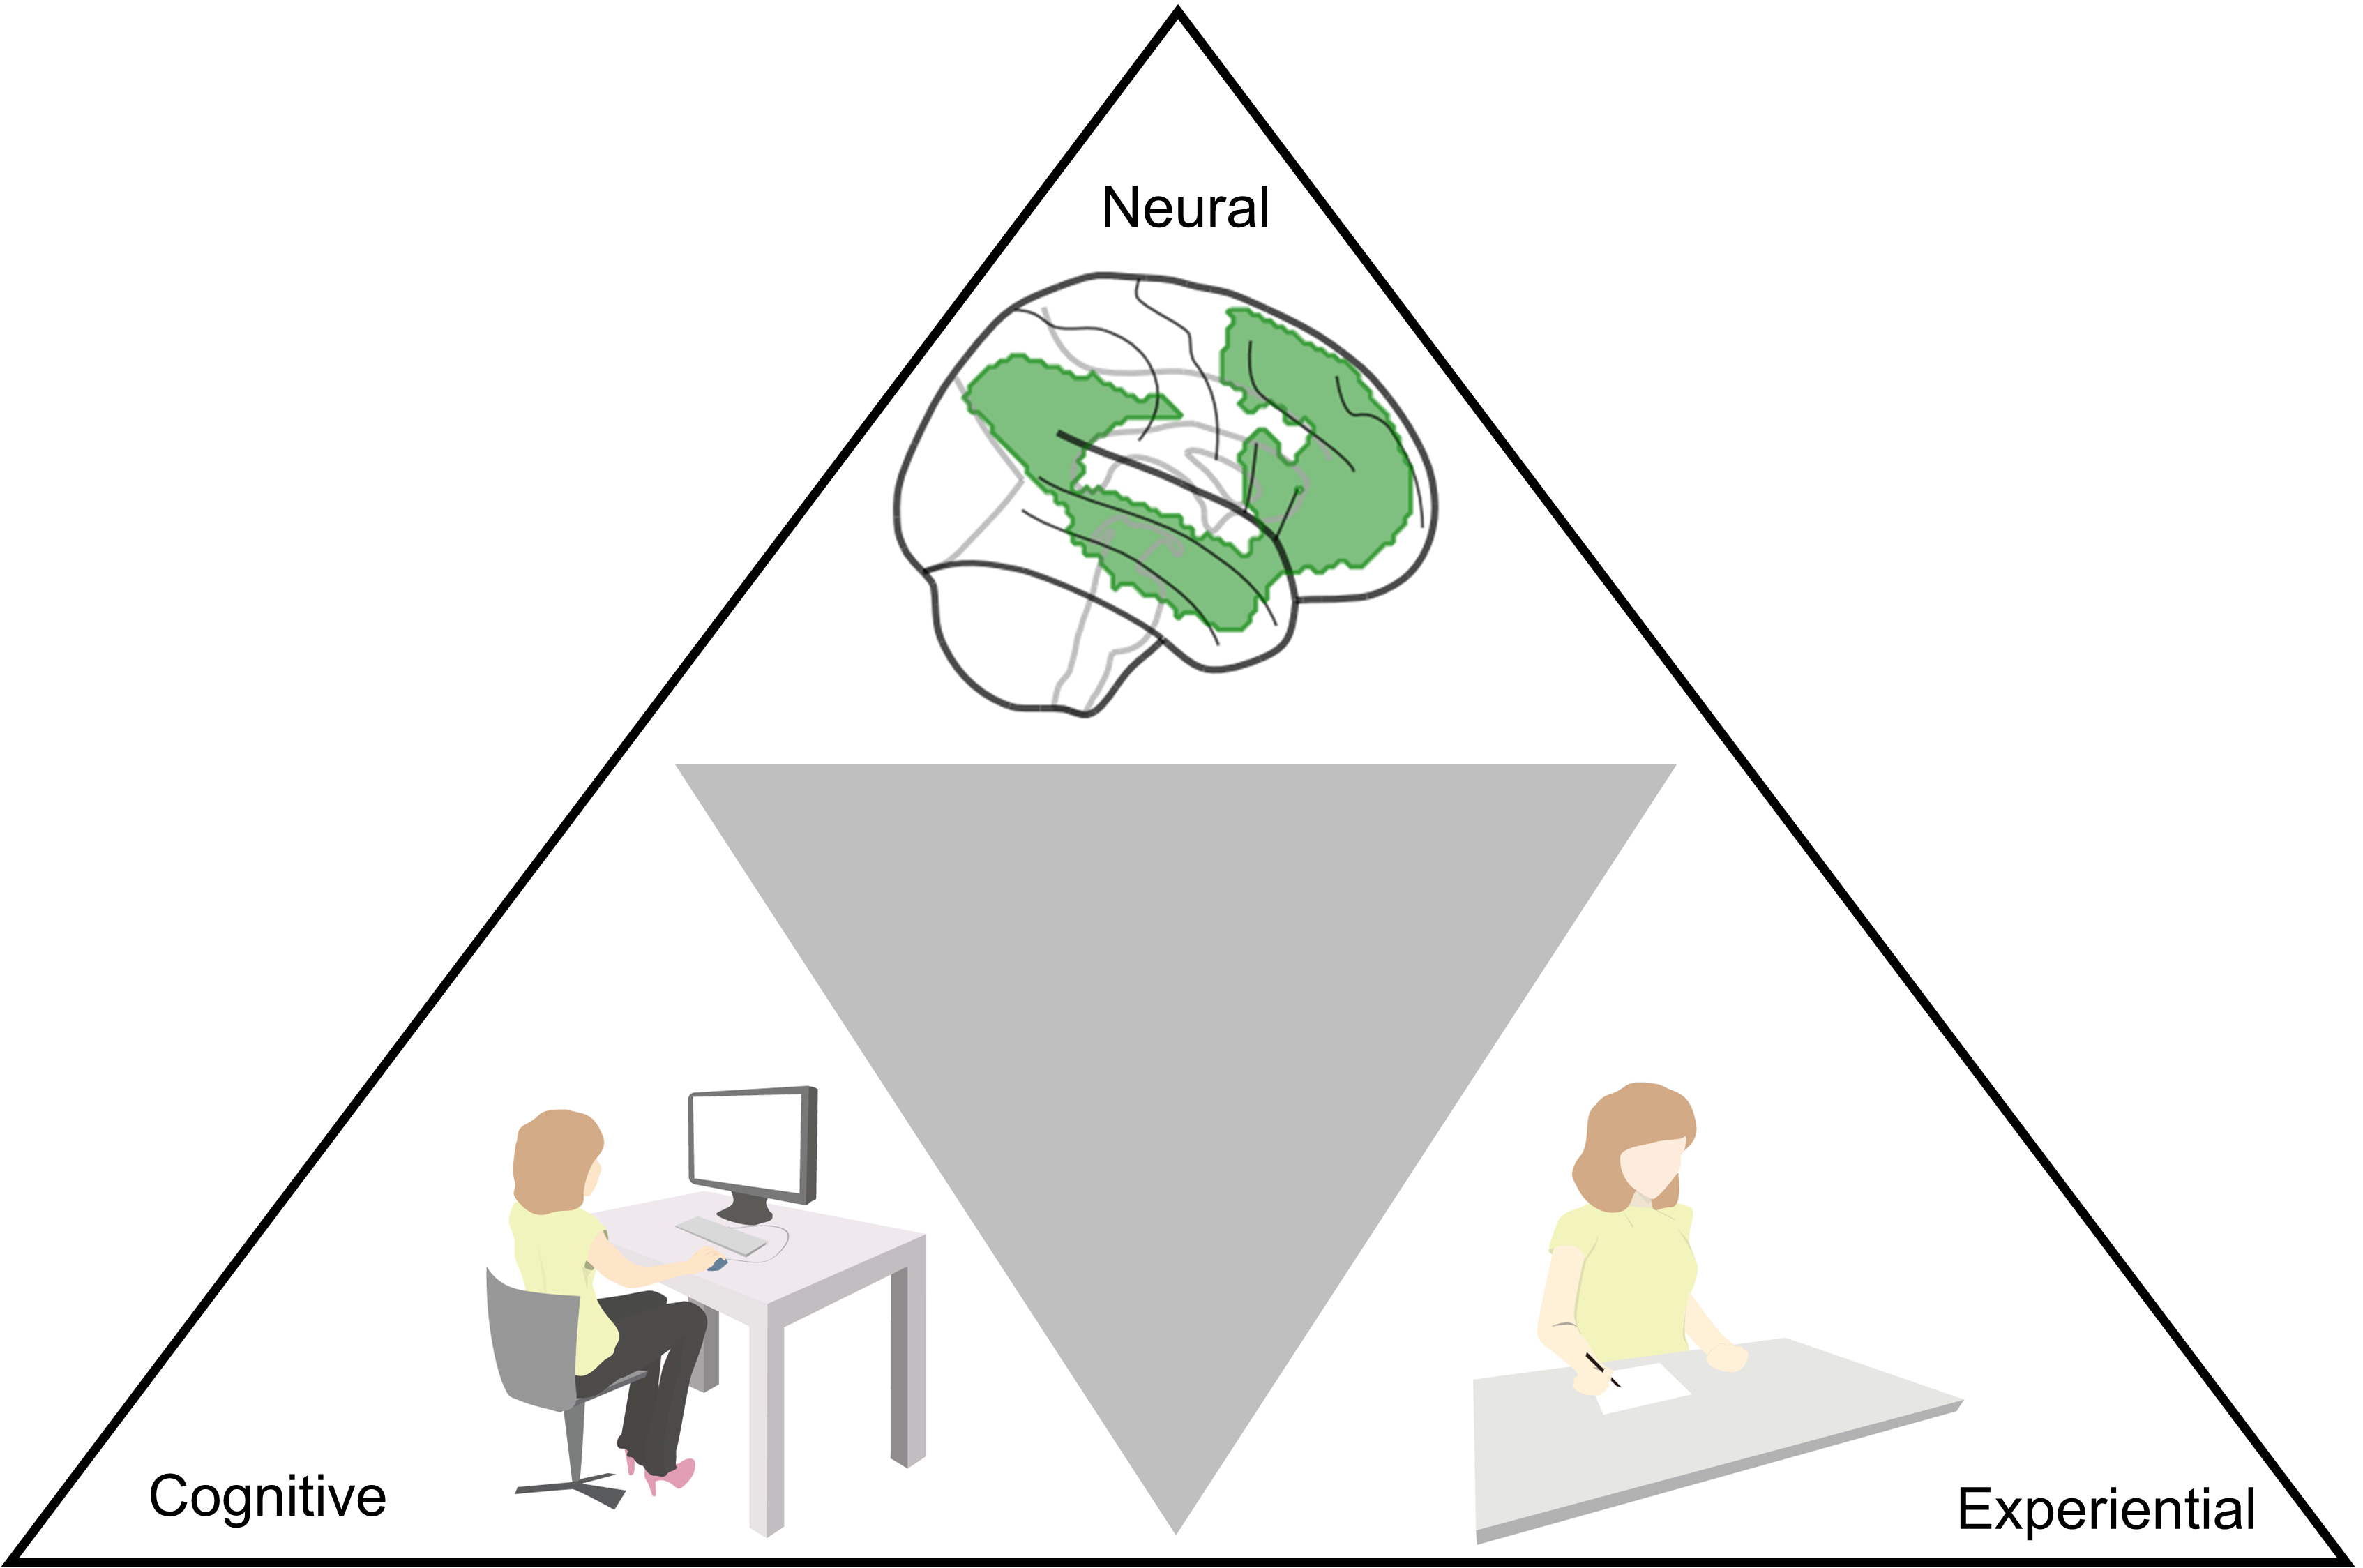
\includegraphics[width=0.8\textwidth]{intro/image/thesisfig1.png}
	\caption{Schematic of the thesis}
	%\vspace{-10pt}
	\label{fig:intro:fig1}
\end{figure}

Studies targeting relationships of a singular aspect would only capture few potential members of the family of on-going thought. When the family members sampled possess non-prototypical features, the discovery could be presented as rival theories. For instance, the study of on-going thought associated with creativity and working memory are presented as conflicts of mind wandering profiles. With a understanding of the component processes composing the family property, the heterogeneity of on-going thought may be interpreted as exemplars of component processes rather than conflicts. 

The current thesis adapts a multivariate approach as the first step towards a family resemblance view of on-going thought. A multivariate approach can include observations on a wider variety of behavioural profiles, thus preventing over-representing an exemplar as the whole category. Multidimensional experience sampling \cite<MDES; >{Medea2016, RubyPlos2013, Smallwood2016} is the main technique of experience profile assessment to capture the various aspects of thought. Resting state functional connectivity is used to describe the trait-like neural feature of each individual. The tasks selected measure cognitive functions documented in the past mind wandering literature, including executive control, fluid intelligence, episodic memory, semantic memory, and information generation. Finally, canonical correlation analysis \cite<CCA; >{Hotelling1936} is the conjoined-decomposition method of choice to explore the multivariate patterns of mind wandering. Here I present the overview of the on-going thought measure and the benefit of CCA used in the thesis.  

\subsection{Content of experience}

To access the complex, heterogeneous content of spontaneous thoughts, the current thesis employs MDES \cite{Medea2016, RubyPlos2013, Smallwood2016}. For the purpose of capturing momentary evolution of thoughts during experiments, experience sampling \cite{Kahneman2004} is the commonly used technique. MDES expanded the thought probe from a on/off task question to a collection of dimensions related to a wide range of form and content of thoughts. The idea of MDES is based on various questionnaires to understand the content of mind wandering thoughts retrospectively, such as the Dundee Stress State Questionnaire \cite{Matthews1999}, Amsterdam Resting-State Questionnaire \cite{Diaz2013}, the resting state questionnaire \cite{Delamillieure2010}, and New York Cognition Questionnaire \cite{Gorgolewski2014}. The questionnaires above involves more than 20 items, providing a comprehensive coverage of thought content. Direct implementation of the retrospective questionnaires listed above is not practical for experience sampling. Experience sampling is conducted along an external task, such as reading \cite{Franklin2011}, go/no-go task \cite{Christoff2009}, and n-back task\cite{Kane2007}. The list of questions need to be short and concise to minimum interruption of the external task. 

The current version of MDES is based on 10-question set used in \cite{Medea2016} and \citeA{Smallwood2016}. In the previous work, the questions are separated into content and form aspect of experience. PCA was used to extract latent linear structure in the spontaneous thought report. Each participant has a set of identified principle components concluding the average momentary state of all the sampled time period. The current version includes both form and content questions in one set with three extra questions. The average score of each thought dimension indicate the average momentary state of on-going thought. Unique associations among the questions are expected to capture the family resemblance at a experiential level. 

\subsection{Method of acquiring experience}

In the current thesis, both online and retrospective method are used to acquire content of mind wandering in laboratory scenario. In the second empirical study, New York Cognition Questionnaire \cite{Gorgolewski2014} is used to acquire the trait-like multidimensional mind wandering thought content during a 9-minute resting state fMRI session. The retrospective method measures the summary of the mind-wandering experience during a specified time period. The benefit of retrospective measure is that no interruption during the given task or the on-going thoughts will happen. The trait-level features of mind wandering are accessed in the retrospective report. 

In the online measure, MDES serves as the thought probes to record participant's experiences during a give task. Thought probe appears during the task in a semi random fashion. The online measure captures spontaneous thought in, possibly, both mind-wandering and task-focused moments. In the first and third empirical studies, the averaged momentary report from MDES is used to capture the trait-like feature of spontaneous cognition.

% A hybrid of go/no-go task and n-back task was used to manipulate working memory capacity to induce mind wandering \cite{Konishi2015, Medea2016}. The earlier version has used number as the test items \cite{SmallwoodNI2013,SmallwoodPlos2011}. The majority of the experiment consist of nontarget presented in neutral colour and a small proportion of targets. The participant are instructed to judge whether the target number is odd or even. In the \textit{choice reaction time} (i.e. 0-back) condition, the judgement is made when the number changes colour; in the \textit{working memory} (i.e. 1-back) condition, participants judge the number on the previous screen when presented with a question mark. The improved version is proposed by Konishi and colleagues \citeyear{Konishi2015}, replacing number with two 2-dimensional geometric shapes separated by a vertical line. Each pair consists of a two shapes among a circle, a triangle, and a square, each in two different left/right configurations. In the 0-back condition, the target is flanked by one of two shapes, and participants indicate which shape matches the target shape. In the 1-back condition, the target is flanked by two question marks, and participants match the target shape to the prior trial. 

\subsection{Conjoined decomposition of brain and cognition}

Despite invented in the 30s, CCA has not aroused researchers’ interests due to the lack of practicality. With the advance on computing resource and enriched data size, CCA has gained popularity in neuroimaging research. Three characteristic of CCA make it the choice of method---joint information compression, symmetry, and multiplicity (details described in \cref{ch:methods}). CCA can be understood as a natural extension of PCA to two variable sets, but mutually linked by a joint correlation criterion. Such extension enables the exploration of neuro-experiential component processes of the on-going thought family. CCA does not distinguish between the two variable sets during the information compression process. The identified dual-component dimensions correlates two aspect the data together without indication of causality between neural function and cognition. CCA is capable of estimating more than one corresponding component pair from the two variable sets. More than one pair of meaningful decomposition can be found, giving it the potential to examine the heterogeneity of mind wandering content and their functional outcome. 

While CCA provided useful features to explore on-going thought, its sparsity variation overcomes two technical issues of CCA application. Performing feature selection with sparsity improve the interpretability of the data and model fit. The data with more number of features than samples is accompanied with consequences of the so-called curse of dimensionality---the more dimensions are added to a data set, the less explanatory value a sample would have \cite{Domingos2012}. The number of functional connectivity measure can easily exceed the number of samples. In sum, SCCA allows decomposition on functional connectivity measures without sacrifice of data richness or interpretation difficulty of prior data compression. The pros and cons of CCA and its variation is disccussed in the next chapter.

The current thesis adopt the sparse variation of CCA \cite<SCCA; >{WittenSCCA2009} to resolve arguments related to the component processes under the family resemblance view. Most studies of on-going thought have only focused on its relationship with one cognitive outcome at a time. As a consequence, mind wandering is treated as a singular construct of all off-task on-going thought. Studies on contents of on-going experience have shown the diversity of information using self-report methods. Based on the heterogeneity of content, on-going thought can be a collection various type of spontaneous thoughts. Adopting multivariate method has the potential to identify family resemblance among the heterogeneity of on-going thought, and to begin the research on the ontology of the component processes of on-going thought. 

% ==========================================================================================================
\section{Summary and thesis outline}
\sectionmark{Summary}
Human cognition has the capacity to generate thoughts loosely related to the external world. However, researchers have not understood the mechanism behind the consequences of on-going thought. The heterogeneity of functional outcomes has been a controversial and much disputed subject within the field of mind wandering research. Extensive research has shown that both cost and benefit to cognitive functions are associated with mind wandering. Negative consequences include reduced attention, poor task performance, unhappiness, and depression. The related positive outcomes include creative problem solving, planning personal goals, and recovery from negative emotion. 

Most studies in mind wandering have only focused on one cognitive outcome at a time. Mind wandering is treated as a singular construct. Studies on contents of spontaneous on-going thoughts have shown the diversity of information using self-report methods. The temporal content of on-going thoughts can be future- or past-focused. The topic can be on personal issues or task related. Based on the heterogeneity of content, on-going thoughts can be a family of various type of spontaneous thoughts with essential shared features. The lack of understanding in family resemblance component processes result in conflicts in on-going thought literature.

In the past decade, the neural basis of unconstrained processes has become the centre of the topic. DMN is the commonly emerged large-scale network. Extensive literature have documented the task-negative trait of DMN. The executive failure account of mind wandering is in line with the task-negative view of DMN. However, the memory representation aspect of the on-going thought mystery is left unresolved. Recent literature on the neural hierarchy has shade a different light on the function of DMN. The high-level cognitive functions are associated with DMN, whereas perception and motor related regions are related to low-level tasks. This new view provides a clue to investigate the representational account of on-going thought. 

The conflict in mind wandering literature is related to the one-to-one matching between on-going thought and the brain or behaviour. To paint the full picture of on-going thought, a multivaritate method will help incorporate the three aspects mentioned above: cognition, experience, and neural basis. The current thesis adopt SCCA to resolve arguments related to heterogeneity in mind wandering. Despite invented in the 30s, CCA has not aroused researchers’ interests due to the lack of practicality. With the advance on computing resource and enriched data size, CCA has gained popularity in neural imaging research. The motivation of the current thesis is to resolve the conflict in on-going thought literature incorporating functional organisation of large-scale neural networks. The aim is to present evidence supporting of the family resemblance view, and to begin research on the ontology of the component processes in on-going thought. A outline of the remaining chapter is listed below: 

\subsection*{Canonical correlation analysis}

Canonical correlation analysis is introduced as the main method of the thesis. This review focuses the potential applications in neuroimaging research. The features, applications of this multivariate method are outlined, followed by discussion on the method's the interpretations and limitations. 

\textit{This chapter is under preparation for publication. } 

\subsection*{Exploring the heterogeneity of on-going thought}
Heterogeneity of mind wandering leads to conflicts in its functional outcome in behavioural study. Default mode network is commonly associated with the emergence of mind wandering. SCCA conjointly decomposed functional connectivity patterns of DMN and thought reports, revealing unique neuro-experiential components. The study then revealed that the neuro-experiential components each associate with unique cognitive task measures. The various connectivity configuration within DMN is associated with different types of on-going thought and their specific functional outcomes.

\textit{This chapter is published in Psychological Science.}

\subsection*{Population variation in the associations between large-scale network and experiences}
Unconstrained cognitive processes have two faces. The representational account argues that the primary sensory brain region decoupling from the DMN to facilitate memory representation; whereas the executive failure account shows lapses in attention is related to the demand to attention system and activation of DMN. We used SCCA to extract related whole brain functional connectivity patterns, profiling the neuro-experiential components of unconstrained cognitive processes. Examining the association between demanding cognitive tasks and neuro-experiential components, the study revealed evidence supporting both the representational and executive failure accounts.

\textit{This chapter is published in NeuroImage.}

\subsection*{Inhibition of prior information contributes to internal content representation}
Various cognitive function is involved in the generation of internal experiences. The study of the functional outcome are often conducted in a manner of one-to-one mapping. The heterogeneous cognitive outcomes are discussed as conflicts rather than the complex details driving the diversity of on-going thought. In the current chapter, we explore the intrinsic whole-brain neural basis of the cognitive functions supporting the unconstrained generation of spontaneous thoughts.  With SCCA we describe the conjoined decomposition of cognitive function and resting state functional connectivity. The study explore the unconstrained neuro-cognitive mechanism underlying the various dimensions of on-going thought.

\subsection*{General discussions}
The overarching themes of the thesis are discussed and linked to specific results throughout the thesis. Future research directions are inspired by the findings and limitations of the current thesis.

% ==========================================================================================================
